\documentclass{article}
\usepackage{amsmath,amssymb}
\usepackage{graphicx}
\usepackage{enumerate}
\usepackage{hyperref}
\usepackage{subcaption}
\usepackage{caption}
\usepackage{xcolor}

\pagestyle{empty} \addtolength{\textwidth}{1.0in}
\addtolength{\textheight}{0.5in}
\addtolength{\oddsidemargin}{-0.5in}
\addtolength{\evensidemargin}{-0.5in}
\newcommand{\ruleskip}{\bigskip\hrule\bigskip}
\newcommand{\nodify}[1]{{\sc #1}}
\newcommand{\points}[1]{{\textbf{[#1 points]}}}
\newcommand{\subquestionpoints}[1]{{[#1 points]}}
\newenvironment{answer}{{\bf Answer:} \sf }{}%

\newcommand{\bitem}{\begin{list}{$\bullet$}%
{\setlength{\itemsep}{0pt}\setlength{\topsep}{0pt}%
\setlength{\rightmargin}{0pt}}}
\newcommand{\eitem}{\end{list}}

\setlength{\parindent}{0pt} \setlength{\parskip}{0.5ex}
\setlength{\unitlength}{1cm}

\newcommand{\pa}[1]{[[PA: #1]]}

\renewcommand{\Re}{{\mathbb R}}
\newcommand{\E}{{\rm E}}
\begin{document}

\pagestyle{myheadings} \markboth{}{CSCI 4302/5302 Advanced Robotics, Homework \#3, Fall 2021}

{\huge
\noindent HW \#3: Motion Planning with RRT}\\
\ruleskip
{\bf Name}: YOUR NAME HERE\\

{\bf Deliverable}:  PDF write-up and code by {\bf Friday October 29th, 5:00pm}.  Your PDF should be generated by replacing the placeholder images in this LaTeX document with the appropriate solution images for each question.  Your PDF and code (hw3\_rrt.py) is to be submitted via the course Canvas. The scripts will automatically generate the appropriate images, so you only need to recompile the LaTeX document to populate it with content.

\textbf{Graduate Students:} You are expected to complete the entire assignment.\\
\textbf{Undergraduate Students:} You need only complete questions that do not have \textbf{(GRAD)} next to them.\\

\vspace{.1in}

To generate figures, you will need to have matplotlib:\\
pip install matplotlib (you should have this from your previous assignment)\\


\newpage
%--------------------------------------------------------------------------------
%--------------------------------------------------------------------------------
%--------------------------------------------------------------------------------
\noindent {\bf 1. Rapidly-Exploring Random Trees}
%--------------------------------------------------------------------------------
%--------------------------------------------------------------------------------
%--------------------------------------------------------------------------------

\begin{enumerate}[(a)]
\item {\bf [30pts] RRT.} First, you will implement the RRT algorithm for holonomic robots on the X-Y plane. You will need to put your code in \texttt{code/hw3\_rrt.py} in the function \texttt{rrt}. You will also need to add your own code to implement the general-purpose \texttt{get\_nearest\_vertex} and \texttt{steer\_holonomic} functions (any valid implementation will do). Make sure the figures generated from the two provided 2D obstacle worlds look reasonable and appear below.

\begin{figure}[h!]
    \centering
    \begin{subfigure}{0.45\textwidth}
        \centering
        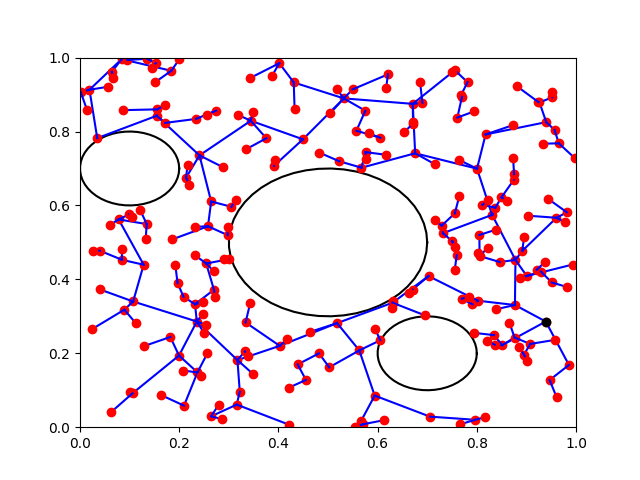
\includegraphics[width=\textwidth]{../figures/rrt_run1.png}
        \caption{RRT from the First 2D Domain}
    \end{subfigure}
    \hspace{0.2in}
    \begin{subfigure}{0.45\textwidth}
        \centering
        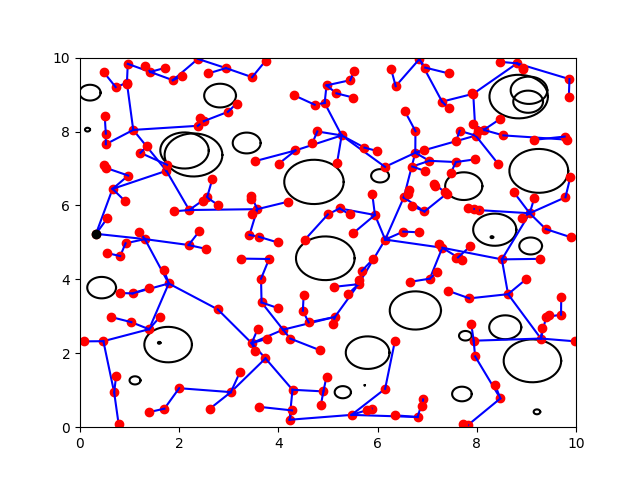
\includegraphics[width=\textwidth]{../figures/rrt_run2.png}
        \caption{RRT on a Random 2D Domain}
    \end{subfigure}
\end{figure}

\begin{figure}[h!]
    \centering
    \begin{subfigure}{0.45\textwidth}
        \centering
        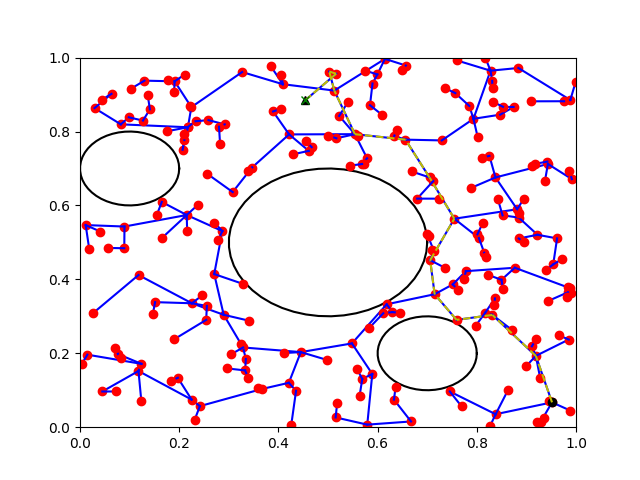
\includegraphics[width=\textwidth]{../figures/rrt_run3.png}
        \caption{Goal-Directed RRT on the First 2D Domain}
    \end{subfigure}
    \hspace{0.2in}
    \begin{subfigure}{0.45\textwidth}
        \centering
        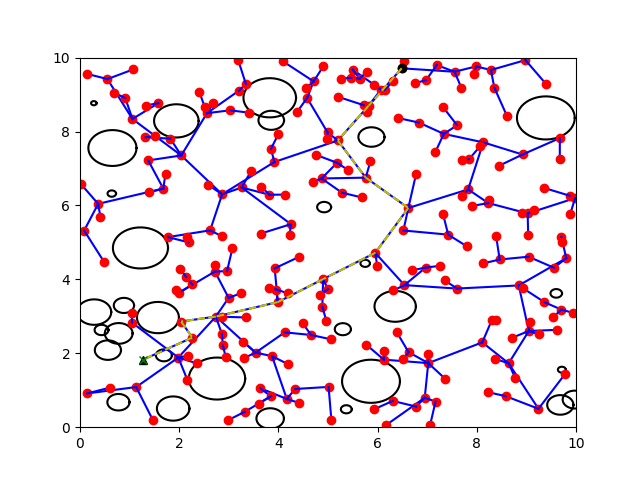
\includegraphics[width=\textwidth]{../figures/rrt_run4.png}
        \caption{Goal-Directed RRT on a Random 2D Domain}
    \end{subfigure}
\end{figure}


\item {\bf [50pts] RRT*.} Implement the RRT* algorithm for holonomic robots on the X-Y plane. You will need to put your code in \texttt{code/hw3\_rrt.py} in the function \texttt{rrt\_star}. Make sure the figures generated from the two provided 2D obstacle worlds look reasonable and appear below.

\begin{figure}[h!]
    \centering
    \begin{subfigure}{0.3\textwidth}
		\centering
		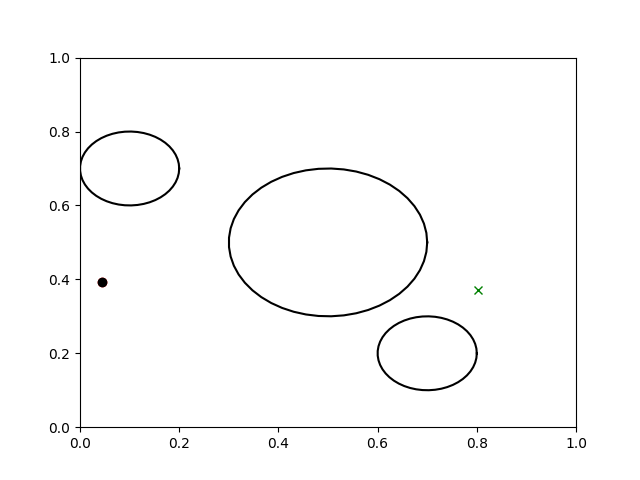
\includegraphics[width=\textwidth]{../figures/rrt_star_run1-empty.png}
		\caption{Planning Domain}
	\end{subfigure}
	\hspace{0.05in}
    \begin{subfigure}{0.3\textwidth}
        \centering
        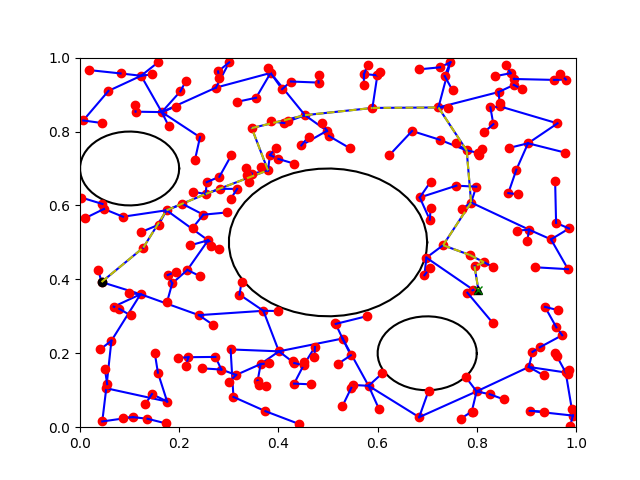
\includegraphics[width=\textwidth]{../figures/rrt_comparison_run1.png}
        \caption{RRT on the First 2D Domain}
    \end{subfigure}
    \hspace{0.05in}
    \begin{subfigure}{0.3\textwidth}
        \centering
        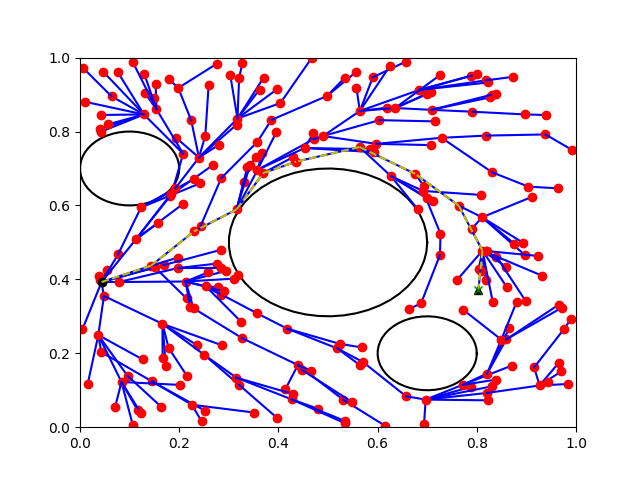
\includegraphics[width=\textwidth]{../figures/rrt_star_run1.png}
        \caption{RRT* on the First 2D Domain}
    \end{subfigure}
\end{figure}

\begin{figure}[h!]
    \centering
    \begin{subfigure}{0.3\textwidth}
		\centering
		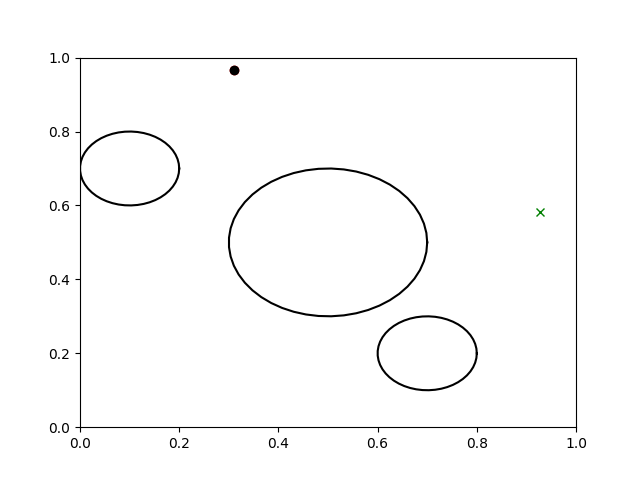
\includegraphics[width=\textwidth]{../figures/rrt_star_run2-empty.png}
		\caption{Planning Domain}
	\end{subfigure}
    \hspace{0.05in}
    \begin{subfigure}{0.3\textwidth}
        \centering
        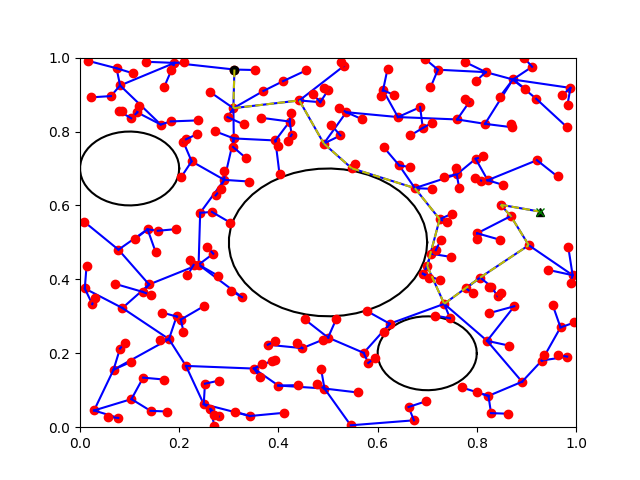
\includegraphics[width=\textwidth]{../figures/rrt_comparison_run2.png}
        \caption{RRT on the Second 2D Domain}
    \end{subfigure}
    \hspace{0.05in}
    \begin{subfigure}{0.3\textwidth}
        \centering
        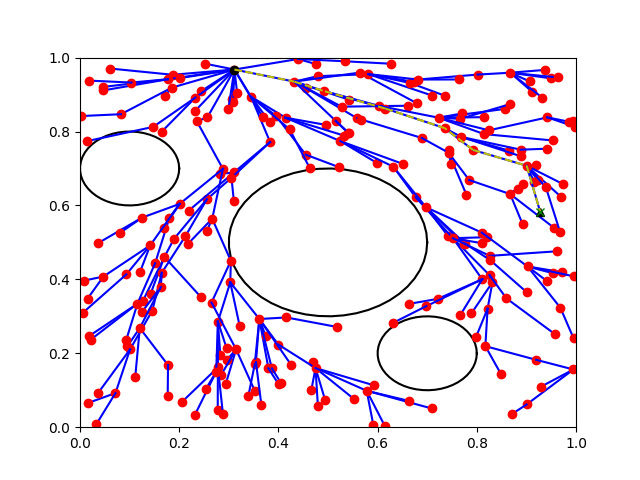
\includegraphics[width=\textwidth]{../figures/rrt_star_run2.png}
        \caption{RRT* on the Second 2D Domain}
    \end{subfigure}
\end{figure}



\item {\bf [20pts] Discrete Non-Holonomic RRT (GRAD).} If our robot cannot freely traverse the coordinate system used in our RRT algorithm, then we can't just add vertices wherever we want and interpolate from existing ones (our robot may not be able to take that path or get there!). Fill in the code for the \emph{steer\_discrete\_non\_holonomic} function that would operate on a discrete action space given as a list \emph{actions\_list}. This agent will only be able to move diagonally!

\begin{figure}[h!]
    \centering
    \begin{subfigure}{0.45\textwidth}
        \centering
        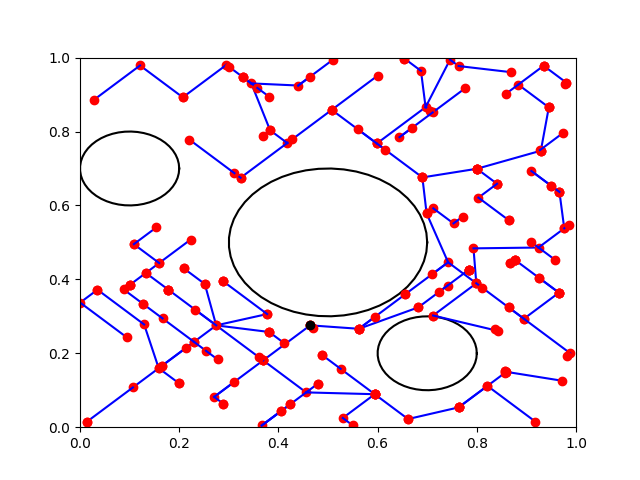
\includegraphics[width=\textwidth]{../figures/rrt_nh_run1.png}
        \caption{RRT with discrete action space}
    \end{subfigure}
    \hspace{0.2in}
    \begin{subfigure}{0.45\textwidth}
        \centering
        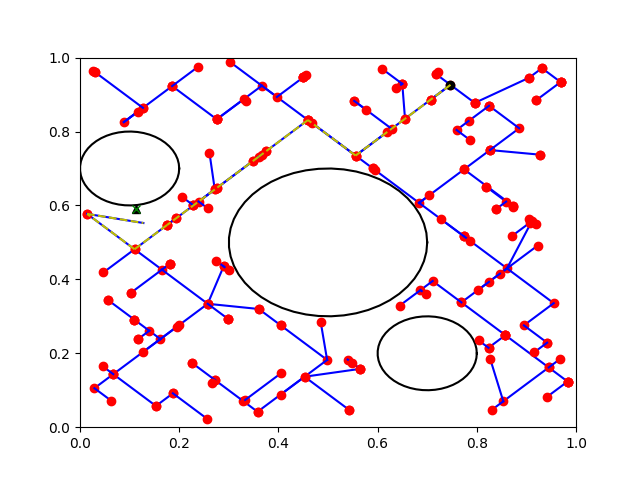
\includegraphics[width=\textwidth]{../figures/rrt_nh_run2.png}
        \caption{RRT with discrete action space}
    \end{subfigure}
\end{figure}


\end{enumerate}


\end{document}
